\chapter{Simulation}\label{cha: Simulation}

In this section, simulations are performed using real-life data to evaluate the performance of the proposed energy management policy. In the experiments, the hourly residential load $x_d(h)$, for $h=1,\ldots, H$, is based on the average hourly load data of a class of residential single families with electric space heat delivery (The definition can be found in ComEd's electronic tariff documents \footnote{Residential Single Family With Electric Space Heat Delivery Class means the delivery class applicable to any retail customer in the residential sector (a) that uses electric service for residential purposes, (b) for which service is provided through a separate meter from an overhead or underground connection that serves no more than two (2) retail customers, and (c) that uses only (i) electric resistance heating devices, (ii) electric-only heat pumps, (iii) solar energy collectors that provide space heating through heat exchangers, or (iv) any combination of the preceding items (i) through (iii) to meet the entire space heating requirements at such retail customer's premises.}) during January 1, 2010 to December 31, 2014, provided by ComEd \cite{comed:}. In Figure~\ref{fig: x2010}, we can see that the residential load in the winter (January, February, and December) in 2010 is higher then other season in 2010 because of the electric space heat delivery. The day-ahead electricity price is based on the data from January 1, 2010 to December 31, 2014 provided by the ComEd RRTP program \cite{comed:}. In Figure~\ref{fig: p_RT2010}, we can see that the real-time electricity price in summer (January, February, and December) is more expensive then other season.

\begin{figure}[H]
    \centering
    \includegraphics[width = 0.8\textwidth]{fig/x2010.eps}
    \caption{Average residential load per month in 2010.}
    \label{fig: x2010}
\end{figure}

\begin{figure}[H]
    \centering
    \includegraphics[width = 0.8\textwidth]{fig/p_RT2010.eps}
    \caption{Average electricity price per month in 2010.}
    \label{fig: p_RT2010}
\end{figure}

\begin{figure}[H]
    \centering
    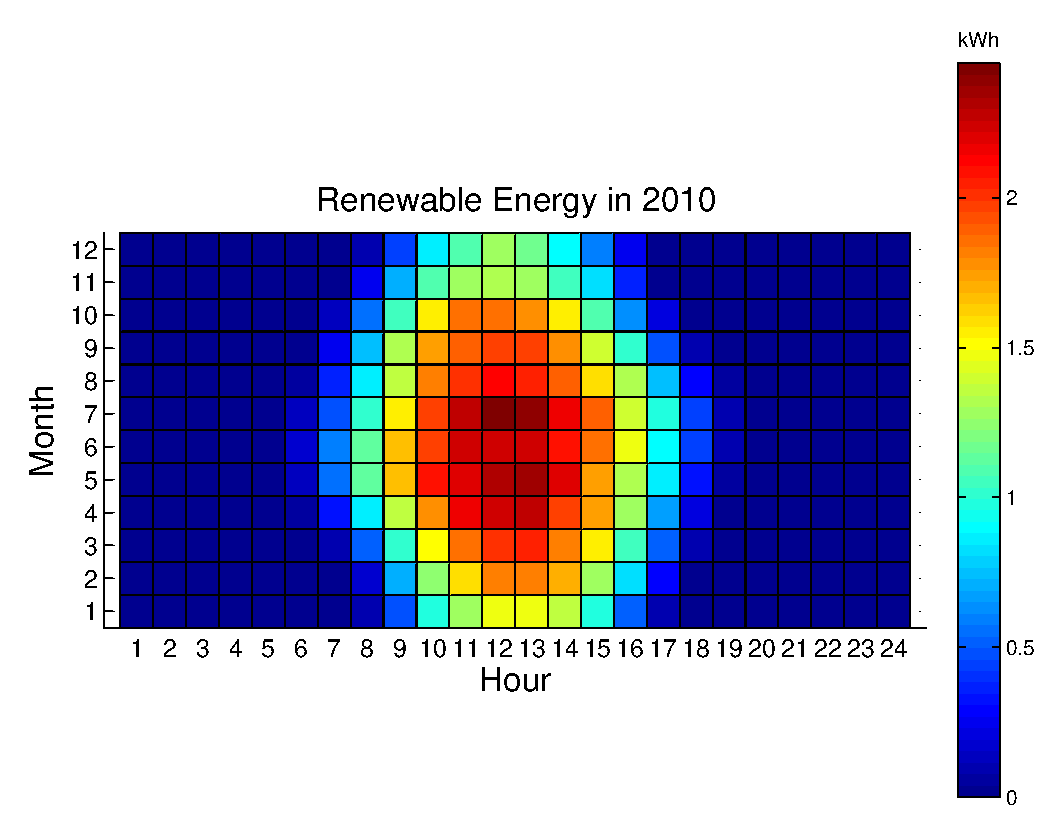
\includegraphics[width = 0.8\textwidth]{fig/r2010.eps}
    \caption{Average renewable energy arrival (solar panel) per month in 2010.}
    \label{fig: r2010}
\end{figure}

Note that the concept of day-ahead purchase has not yet been adopted in practice in the residential setting. The day-ahead electricity price given by \cite{comed:} is actually a prediction of real-time electricity price that the company gives the consumer for reference. In our simulations, we take $80\%$ of the day-ahead electricity price given by \cite{comed:} as the price for day-ahead purchase in our problem. Therefore, the grid cost is given by
\begin{equation}
    \kappa^\text{grid}_d(h) = 0.8 p^\tDA_d(h)\alpha_d(h)+p^\tRT_d(h)\beta_d(h)+p^\text{DP}_d(h)\delta_d(h).
\end{equation}
Moreover, we assume that renewable energy is obtained from photo-voltaic (PV) solar panels and the energy arrival is computed using the NREL PVWatts Calculator \cite{nrel:} with Chicago's public weather data (TMY2, TMY3). The size of the PV panel is $25$ m$^2$. Here, we set $H=24$ and $p^{\text{DP}}_d(h) = 0.5$ Cent per kWh. In Figure~\ref{fig: r2010}, we can see that the hours of sunshine in summer is more than winter.


In the LSPI, the data from the first year, i.e., 2010, along with actions obtained from equal cost policy and 6 random policy are used as the training data samples. In the equal cost policy, the action at time $h$ of day $d+1$ is chosen as
\begin{equation}\label{eq: equal cost policy}
    \alpha_{d+1}(h) = \frac{1/\hat{p}^\text{DA}_{d+1}(h)}{\sum_{h_2=1}^{24} 1/\hat{p}^\text{DA}_{d+1}(h_2)}\sum_{h_1=1}^{24}(\hat x_{d+1}(h_1)-\hat r_{d+1}(h_1))
\end{equation}
so that the anticipated cost is equal in each time slot. In the random policy, the action at time $h$ of day $d+1$ is chosen as
\begin{equation}
    \alpha_{d+1}(h) \sim \calU(\mu^\text{LSPI}_{d+1}(h) - 1.5\sigma^\text{LSPI}_{d+1}(h), \mu^\text{LSPI}_{d+1}(h) + 1.5\sigma^\text{LSPI}_{d+1}(h))
\end{equation}
where $\mu^\text{LSPI}_{d+1}$ is the mean of action of all LSPI policy before day $d+1$ at time slot $h$ and $\sigma^\text{LSPI}_{d+1}$ is the stander deviation of action of all LSPI policy before day $d+1$ at time slot $h$. The discount factor is $\gamma=0.9$. The proposed algorithm is summarized in Algorithm~\ref{algo: EMS-LSPI}.

\begin{figure}[t]
  \centering
  \includegraphics[width = 0.8\textwidth]{fig/av_cost.eps}
  \caption{Average cost per year versus different battery sizes.}
  \label{fig: av_cost}
\end{figure}

In Figure~\ref{fig: av_cost}, the average cost per year is shown for 5 different policies, namely, (i) equal cost, (ii) LSPI without DoD considerations, (iii) LSPI with DoD considerations (i.e., the proposed scheme), (iv) perfect prediction for LSPI without DoD consideration, and (v) perfect prediction for LSPI with DoD consideration policies. In (ii) and (iv), the policy is determined by using LSPI independently of the battery cost; in (iv) and (v), the policy is determined with perfect prediction of the next state and, thus, serves as a lower bound to the achievable performance. We can see the proposed LSPI with DoD considerations provides significant reduction in energy cost per year compared to policies (i) and (ii) that do not take into consideration the battery cost due to DoD. However, when there is prediction error, the policies become more conservative in their actions, even in the without DoD case. Therefore, when there is prediction error, the battery cost for the without DoD case does not increase so drastically as the battery size increases. In Figure~\ref{fig: av_cost_batt}, we can see that we have significant performance improve in battery cost while LSPI takes into consideration the battery cost due to DoD. In Figure~\ref{fig: av_cost_grid}, we expect that the police use more less grid since it is independently of the battery cost in without DoD case. Being conservative helps prevent deep discharge in the without DoD case when there is prediction error. However, in the without DoD case, it may still discharge more frequently than the with DoD case. In the case with prediction errors, the without DoD case may discharge prematurely, causing its grid cost to also be higher. However, in the with DoD case, the battery does not discharge as deeply as in the without DoD case and, thus, saves energy in the battery for use when the price is unexpectedly high.

\begin{figure}[H]
  \centering
  \includegraphics[width = 0.8\textwidth]{fig/av_cost_batt.eps}
  \caption{Average battery cost per year versus different battery sizes.}
  \label{fig: av_cost_batt}
\end{figure}

\begin{figure}[H]
  \centering
  \includegraphics[width = 0.8\textwidth]{fig/av_cost_grid.eps}
  \caption{Average grid cost per year versus different battery sizes.}
  \label{fig: av_cost_grid}
\end{figure}

In Figures~\ref{fig: total_cost_1} and \ref{fig: total_cost_2}, we shown the total cost with different battery size in $5$ years. We can see that total cost in 5 different policies are increase rapidly from $3$-th years to $5$-th years because of the variation electricity price in $5$-th year is highest then others and variation electricity price in $3$-th year is lowest then others.

In Figure~\ref{fig:num_of_batt}, we show the number of battery replacements that are needed in a $10$ year period versus the battery parameter $c_2$. The $10$ year period includes real data from 2011 to 2014 (with 2010 and 2011 as training data) and also $5$ years of synthesized data obtained with random linear combinations of the data from 2010 to 2014. The battery size is fixed as $C=4$ kWh. We can see that the number of battery replacement increases as the parameter $c_2$ decreases since the number of cycles decreases faster with DoD in this case. Moreover, the proposed LSPI with DoD considerations successfully prolongs the lifetime of batteries compared to other schemes.

In Figure~\ref{fig:av_cost_c2}, we show the average cost per year versus the battery parameter $c_2$. The battery size is fixed as $C=4$ kWh. We can see that the average cost increase as the parameter $c_2$ decrease since the battery cost is increase faster with DoD in this case. This result is with respect to the increase of the number of battery replacement since since the number of cycles decreases faster with DoD. In Figure~\ref{fig:av_cost_p_batt}, the parameter is changed to $p^\text{batt}$. We can see that the average cost per year is increase when battery price increase since the cost of each battery replacement is increase.

\begin{figure}[t]
  \centering
  \includegraphics[width = 0.8\textwidth]{fig/total_cost_1.eps}
  \caption{Total cost with battery size $C = 1$ (kWH) versus different years.}
  \label{fig: total_cost_1}
\end{figure}

\begin{figure}[t]
  \centering
  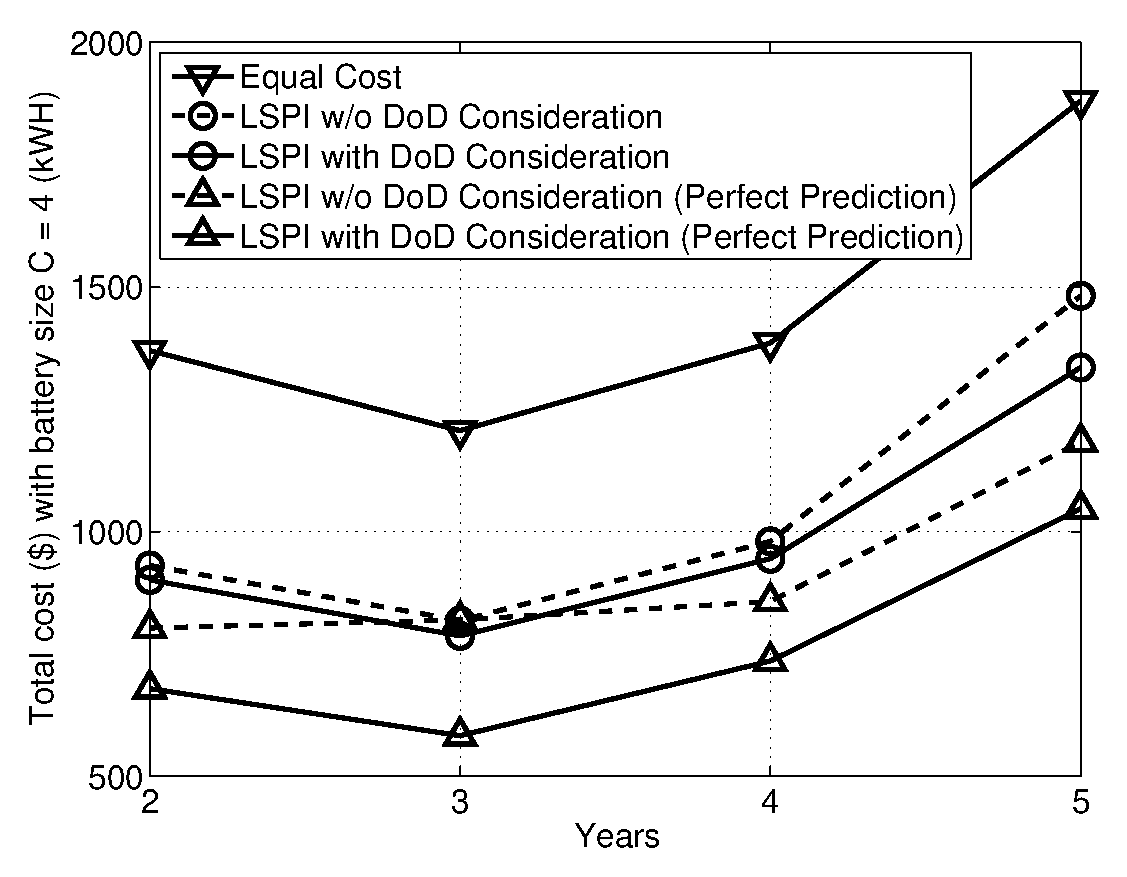
\includegraphics[width = 0.8\textwidth]{fig/total_cost_2.eps}
  \caption{Total cost with battery size $C = 4$ (kWH) versus different years.}
  \label{fig: total_cost_2}
\end{figure}

\begin{figure}[t]
  \centering
  \includegraphics[width = 0.8\textwidth]{fig/num_of_batt.eps}
  \caption{Number of battery replacements versus different values of $c_2$.}
  \label{fig:num_of_batt}
\end{figure}

\begin{figure}[t]
  \centering
  \includegraphics[width = 0.8\textwidth]{fig/av_cost_c2.eps}
  \caption{Average cost per year versus different values of $c_2$.}
  \label{fig:av_cost_c2}
\end{figure}

\begin{figure}[t]
  \centering
  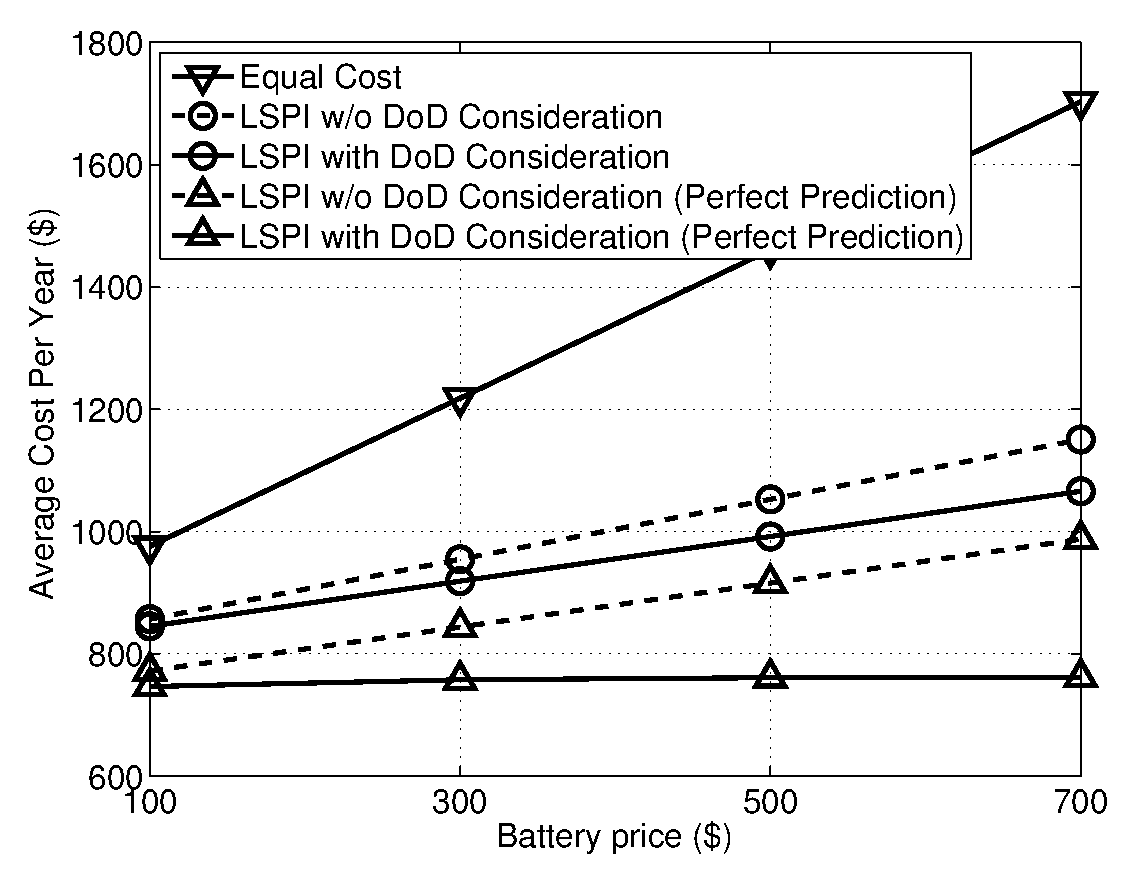
\includegraphics[width = 0.8\textwidth]{fig/av_cost_p_batt.eps}
  \caption{Average cost per year versus different values of battery price $p_\text{batt}$.}
  \label{fig:av_cost_p_batt}
\end{figure}
